\documentclass{report}

\usepackage[backend=bibtex]{biblatex}
\usepackage{graphicx}
\usepackage{lmodern}
\usepackage{minted}
\usepackage{multirow}
\usepackage{subcaption}
\usepackage{tabularx}
\usepackage{tcolorbox}
\usepackage{hyperref}
\usepackage[toc]{glossaries}

\newcommand{\code}[1]{\textsf{\ttfamily #1}}
\renewcommand{\glstextformat}[1]{\textit{#1}}
\addbibresource{Rtutorial.bib}
\makenoidxglossaries

\newglossaryentry{dv}{name={discrete variable}, plural={discrete variables}, description={A variable that refers to categorical data (ex. color of eyes), as opposed to continuous data (ex. height in mm)}}

\newglossaryentry{cv}{name={continuous variable}, plural={continuous variables}, description={A variable that refers to continuous data, i.e. that can take on an infinite number of values (ex. height in mm), as opposed to categorical data (ex. color of eyes)}}

\newglossaryentry{ov}{name={ordinal variable}, plural={ordinal variables}, description={A qualitative variable where the values can be ordered (ex. small, medium, large)}}

\newglossaryentry{qtv}{name={quantitative variable}, plural={quantitative variables}, description={A variable that is measured with numbers (ex. number of cases, height in mm)}}

\newglossaryentry{qlv}{name={qualitative variable}, plural={qualitative variables}, description={A variable that is recorded with words rather than numbers (ex. color of eyes, state of mind)}}

\newglossaryentry{depv}{name={dependent variable}, plural={dependent variables}, description={The "explained" variable in a relationship, the one we try to understand as a consequence of another factor. For example, when studying the effect of smoking on lung cancer, lung cancer is the dependent variable.}}

\newglossaryentry{indv}{name={independent variable}, plural={independent variables}, description={The "explaining" variable in a relationship, the one that drives a phenomena. For example, when trying to understand the causes of diabetes, body mass index would be an independent variable.}}

\author{Myriam Luce}
\title{Statistics with R: a hands-on approach}

\begin{document}
\maketitle
\tableofcontents

\chapter{Data review}
	\section{Possibly interesting extra tidbits}
	In the making of this tutorial, I used several tools that you might like to access as well. Being the tedium-averse programmer I am, I use a reference manager program, in my case Zotero. You can find the full bibliography for this project, including a few entries that did not make it into the references section here because I did not cite them, at \href{https://www.zotero.org/groups/2223910/r_tutorial}{the Zotero project page}.
	
	I also want to point out \href{https://github.com/awesomedata/awesome-public-datasets}{awesome-public-datasets}, where I foraged for the examples in this tutorial. It has several interesting datasets in the public health domain.

	\section{Variables}
	When "doing science", you will be taking measurements, usually in the hopes of understanding a phenomena often in the shape of a relationship between things you are measuring. When working with this data, the nature of the things you measure (\emph{variables}) will influence the presentation and analysis that are appropriate.
	
	A \gls{qlv} refers to categories, or a variable recorded with words, as opposed to a \gls{qtv}, which is measured with numbers. Examples of qualitative variables would include US state, restaurant chains and college major. Quantitative variables could be time to execute a task, waist circumference, disease rate or spending amounts.
	
	R refers to \glspl{qlv} as \emph{factors}. \Glspl{qlv} can further be divided into non ordinal and \glspl{ov}, depending on whether there is a natural order among the categories. For example, dog breed (chihuahua, husky, labrador) is a non ordinal variable, whereas level of satisfaction (dissatisfied, neutral, satisfied) is ordinal.
	
	\Glspl{qtv} are either \glspl{dv}, where measurements are done in integers, or \glspl{cv}, where they come in real numbers (you could get an infinity of decimals with a theoretical instrument of infinite precision). \Glspl{dv} could be number of children, cancer deaths, or wedding age. \Glspl{cv} include temperature, blood sugar level, and weight.
	
	Furthermore, when studying variables in relationship with one another, changes in a \gls{depv} are driven or explained by an \gls{indv}. Typically, this means the "x" axis of a graph will be the \gls{indv}, while the "y" axis will be the \gls{depv}.
	
	\section{Gotchas}
		\subsection{Tidy data}
		When working with data in R, analysis will be easier if your data is \emph{tidy}, that is, each column in your data set contains one and only one variable.
	
		For example, in a cancer dataset that we will use later, the original data is presented as in table \ref{table:cancer}. Here, we have four variables: cancer type, sex, number of cases, and number of deaths. While the first column is one and only one variable, the other columns mix sex with number of cases or sex with number of deaths. If you would like to analyze deaths by sex or cases per cancer type, some data manipulation will be necessary to combine the relevant columns.
		\begin{table}[h]
			\centering
			\begin{tabular}{|c|c|c|c|c|}
				\hline 
				\multirow{2}{*}{Cancer Type} & \multicolumn{2}{c|}{Cases}  & \multicolumn{2}{c|}{Deaths} \\ 
				& Male & Female & Male & Female \\  \hline 
				... &  ... & ...  & ...  & ...  \\ \hline 
			\end{tabular} 
			\caption{Cancer data set format.}
			\label{table:cancer}
		\end{table}

		If you keep your data tidy, R can usually do the combining for you, if you know how to ask nicely. As such, it is recommended that the first thing you do after successfully importing data into R is to verify it is tidy. Tools to divide or merge columns will be discussed in section \ref{sec:data-import}.
	
		\subsection{Correlation is not causation, or of the importance of DoE}
		DoE refers to design of experiments. The common trope that "correlation is not causation" refers to the fact that because two variables vary together does not necessarily mean that one causes the other to change; for instance, they might both be responding to a common cause, when it's not just plain old coincidence. My personal favorite exemplification of "correlation is not causation" is that the divorce rate in Maine correlates with the per capita consumption of margarine \cite{vigen}.
	
		To distinguish between correlation and causation with certainty, a controlled experiment must be run. Depending on the phenomena studied, this might mean using a control group, a placebo, or directly controlling environmental conditions. For example, to determine the effect of low oxygen concentration in water on cod growth, several tanks can be set up where individual cods are randomly distributed and where oxygen levels are controlled. If you were to simply measure oxygen levels in water and cod growth at different locations and subsequently find a correlation between the two, you couldn't tell for certain whether the difference is due to oxygen levels, or another factor like water temperature, or even the fact that cod compete with one another and that the runts, who would grow slower anyway, end up pushed into less desirable low-oxygen environments. Of course, sometimes running a controlled experiment is not feasible for practical reasons (one can't control amount of natural sunlight, for example) or ethical reasons (having an untreated control group of people with a serious condition, when a potentially life-saving treatment might exist, is questionable).
	
		When dealing with humans, to determine whether medication has a positive effect on an health issue, the health issue can be measured for a group who took the medication (treatment group), a group who took a placebo, and a group who took no medication at all (control group). In humans, particular effort must be placed on controlling or measuring the placebo effect, for the test subjects as well as the professionals. A recent spectacular example is the recommendation to abandon arthroscopic surgeries for knee pain because it did not show better results than physical therapy in randomized trials, despite it being the most common orthopaedic procedure in several countries \cite{knee}.
	
		Where experimental design is concerned, key factors are randomization, blocking, and replication. If terms like Completely Randomized Design, Latin Squares or Factorial Design are not familiar, I would recommend investing some time into learning the basics of experimental design before embarking in an experiment, in the interest of avoiding some common and easily remedied mistakes (\cite{doe} appears to be a well-rounded textbook ).

\chapter{Descriptive statistics}
	\section{Data: import, export, tidy}\label{sec:data-import}
		\subsection{R plumbing: packages}
		R \cite{R} should be relatively straightforward to install: download and execute, follow the wizard instructions.
	
		Where things get a bit more complicated is when it comes to packages. While the basic R program has a lot of functions built-in, there will come a time when you will need something that is not offered out of the box. Thankfully, R has a very dynamic community with a ton of packages. For instance, a very popular package to produce figures is ggplot2. Let's install it to see how packages are managed in R.
	
		First off, to install packages in R, you will need to launch it as an administrator. If you don't, you will get the rather unhelpful message shown in figure~\ref{fig:unhelpful}. To launch with administrator rights, right-click on your R launcher and find the option "Run as administrator". How to do so from the Windows 10 start menu is shown in figure~\ref{fig:admin}. (As a note, you should launch as administrator \emph{only} when installing packages, as opposed to modifying your shortcut to always launch as administrator.)
		\begin{figure}[h]
			\centering
			\begin{minipage}{.475\textwidth}
				\centering
				
\includegraphics[width=.8\linewidth]{unhelpful.png}
				\caption{Error message displayed by R if trying to install packages without administrator rights.}
				\label{fig:unhelpful}
			\end{minipage}
			\hfill
			\begin{minipage}{.475\textwidth}
				\centering
				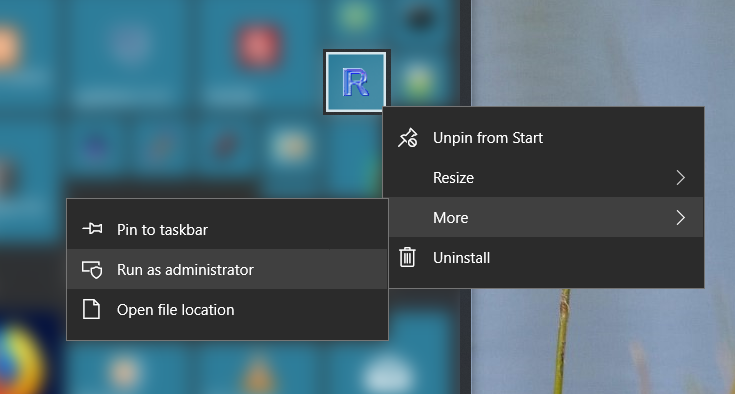
\includegraphics[width=.8\linewidth]{admin.png}
				\caption{How to launch R with administrative rights.}
				\label{fig:admin}
			\end{minipage}
		\end{figure}
	
		Now that R is launched as administrator, you can install ggplot2 using either the convenient Packages menu or the command line if you're that hardcore. Personally I use the menu; after choosing a mirror (different mirrors offer different packages; Canada NS has a wide selection and is vaguely geographically close), you can select your desired package and hit "install", as shown in figure~\ref{fig:install}. Then you only need to wait until R is done doing its thing. If all the lines say "successfully unpacked", all good; otherwise, an error has occurred and you will have to decipher the message to figure out how to remedy the situation. (If you run into any trouble, I would first recommend updating to the latest release of R.)
		\begin{figure}[h]
			\centering
			\begin{subfigure}[b]{0.475\textwidth}
				\centering
				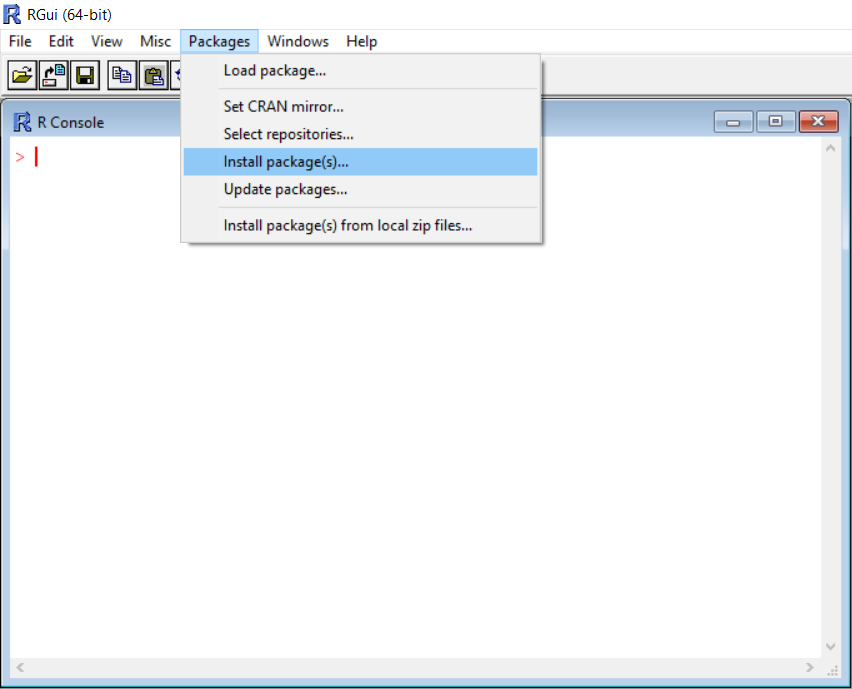
\includegraphics[width=\textwidth]{menu.png}
				\caption{Packages menu in R Gui.}
				\label{fig:menu}
			\end{subfigure}
			\hfill
			\begin{subfigure}[b]{0.475\textwidth}
				\centering
				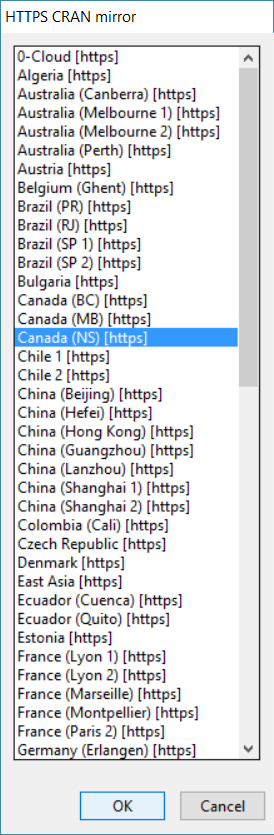
\includegraphics[height=5cm]{mirror.png}
				\caption{List of mirrors.}
				\label{fig:packages}
			\end{subfigure}
			\vskip\baselineskip
			\begin{subfigure}[b]{0.475\textwidth}
				\centering
				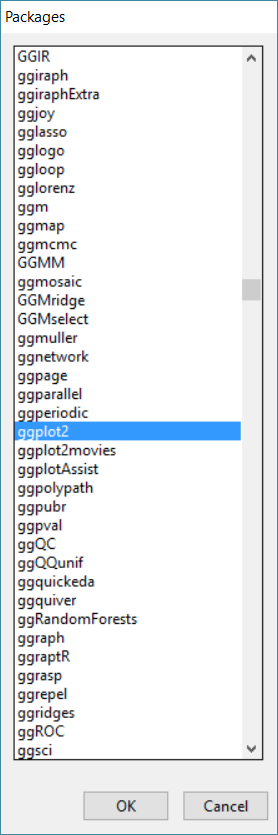
\includegraphics[height=5cm]{packages.png}
				\caption{List of packages.}
				\label{fig:mirror}
			\end{subfigure}
			\hfill
			\begin{subfigure}[b]{0.475\textwidth}
				\centering
				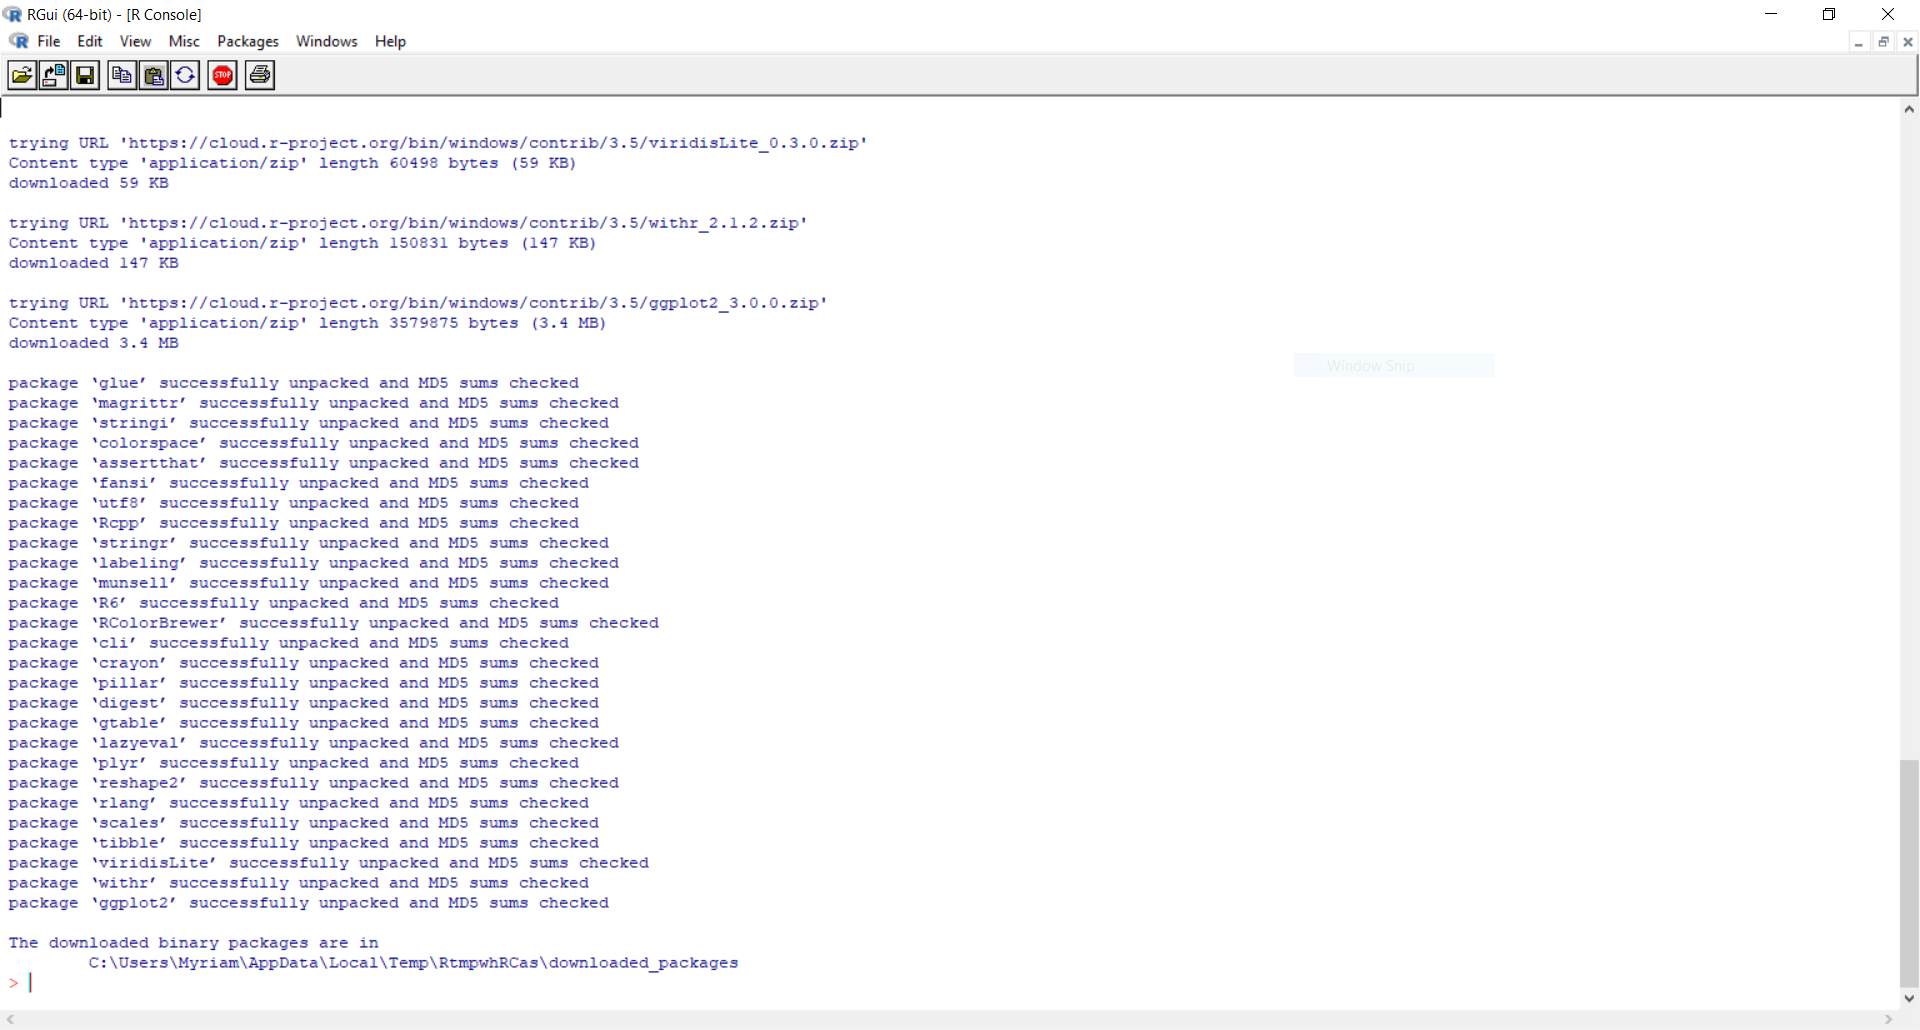
\includegraphics[width=\textwidth]{installed.png}
				\caption{All successfully unpacked: successful installation.}
				\label{fig:installed}
			\end{subfigure}
			\caption{Package installation process.}
			\label{fig:install}
		\end{figure}
	
		Note that installing a package is not enough to use it; you must also load it. Again this can be done either from the menu or with the command line, as shown in figure~\ref{fig:load}. This operation must be repeated \emph{every time} you restart R.
		\begin{figure}[h]
			\centering
			\begin{subfigure}[t]{0.475\textwidth}
				\centering
				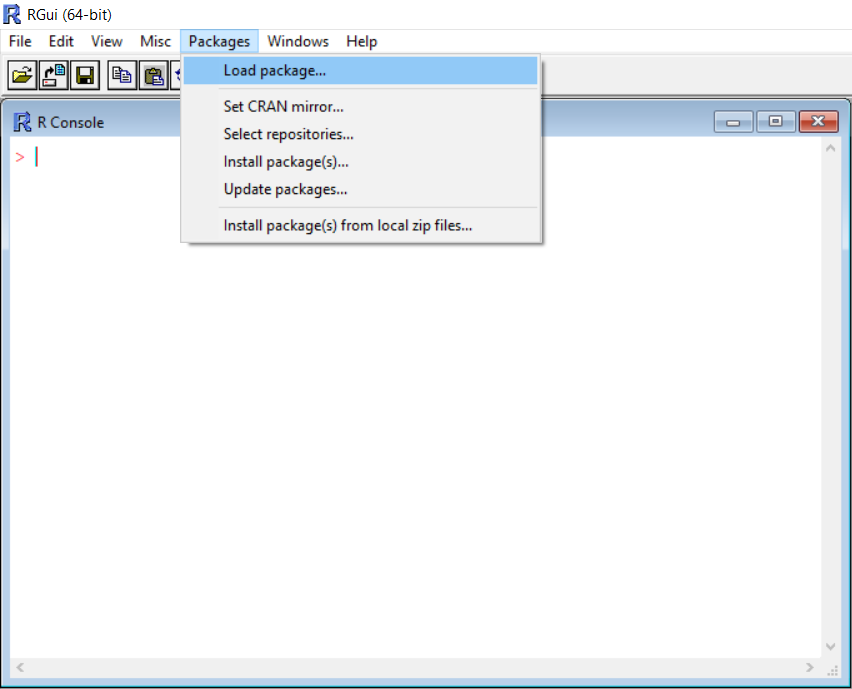
\includegraphics[width=\textwidth]{load.png}
				\caption{Packages menu in R Gui.}
				\label{fig:loadmenu}
			\end{subfigure}
			\hfill
			\begin{subfigure}[t]{0.475\textwidth}
				\centering
				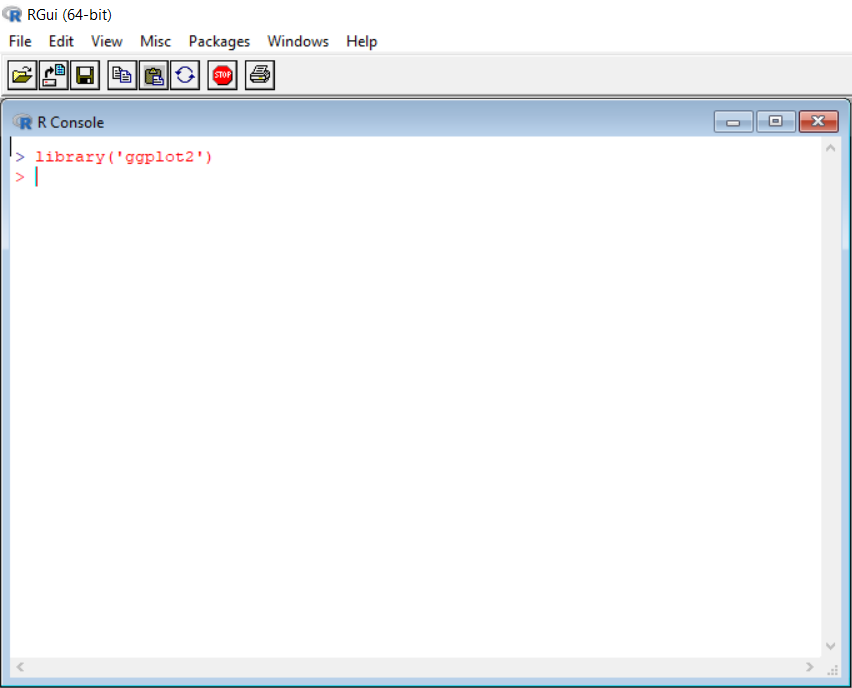
\includegraphics[width=\textwidth]{cli.png}
				\caption{Command to load a package in R Gui.}
				\label{fig:cli}
			\end{subfigure}
			\caption{Loading packages in R.}
			\label{fig:load}
		\end{figure}
	
		Now let's say that \code{ggplot2} becomes your favoritest package in the whole world and you end up using it every day. After a week or so you will probably be very annoyed having to reload the package every time you open R. You can add packages to be loaded automatically in either of two files: \code{Rprofile.site} or \code{.Rprofile}. \code{Rprofile.site} is located in your R installation folder in the etc folder and is always executed. \code{.Rprofile} is located in the user home folder and is applied after the changes made by \code{Rprofile.site}. As the appropriate location to put \code{.Rprofile} seems to change from R version to version, I will showcase the \code{Rprofile.site} here. At the bottom of the file, add the following:
		\begin{minted}[breaklines]{R}
.First <- function(){
	library('ggplot2')
	# other libraries go here
}
		\end{minted}
	
		\subsection{Importing data: \code{read.csv} is your friend}
		A typical workflow to get data from wherever into R would be as follows:
		\begin{enumerate}
			\item Copy-paste the data into your favorite spreadsheet software (Microsoft Excel, LibreOffice Calc, Google Sheets, etc.).
			\item If necessary, transpose your data so that variables are in columns (rather than rows).
			\item Tweak column names so they have no spaces and no special characters (é, \$, etc).
			\item Assign a reasonable format (text, number, thousand separators, etc.) to all columns.
			\item With your operating systems using an English locale, save as csv.
			\item Use \code{read.csv} in R with the appropriate options.
		\end{enumerate}
		Let's cover each of these with a few examples
	
		
		\subsection{Export}
		Exporting data is useful to save it for later use or send to a spreadsheet software. Despite some internationalization issues, I would recommend using csv for the output file, since it is easy to import into spreadsheet software. In that simple case, the \code{write.csv} function works quite well:
		\begin{minted}[breaklines]{R}
> demo
[,1]   [,2]   [,3]   [,4]   [,5]
[1,]  82.94 115.94  89.48 101.06  91.23
[2,] 111.22 117.65  94.64 115.79 103.91
[3,]  82.10  95.96 101.11  82.44  98.84
> write.csv(demo, file='path.../demo.csv', row.names=FALSE)
		\end{minted}
		
		\subsection{Tidy}
		
		\subsection{R plumbing: saving aka scripts}
		As long as you're doing simple things fitting on two or three lines, you probably won't feel the need to "save your file". However, as you start doing more elaborate data treatment or need to document a process used, you will want to save your progress.
		
		One way to save is to use R's built-in \code{workspace}. A \code{workspace} is a \code{.RData} file that contains all the variables (used here in the computer science sense: a value that you attached a name to) you have defined since you started R. For example, if you typed the following:
		\begin{minted}[breaklines]{R}
> 1+2
[1] 3
> a = "I am text"
> x = 5+3
> y = x-8
> x
[1] 8
		\end{minted}
		In this case, \code{a}, \code{x} and \code{y} would be saved in your workspace. Next time you started R, you could load the \code{workspace} and R would know that x is worth 8.
		
		Another useful feature of R is the history, that is, the 250~(by default) last commands you typed in the window. You can access them by pressing the up arrow, which can be pretty handy when you want to tweak a command to fix a typo. You can save it in a \code{.Rhistory} file that you can also load the next time you start R.
		
		Finally, if there is a small routine that you need to save, you can save it in a simple text file that you can load and execute. In the \code{File} menu, choose \code{New script} and type some text in the window, for instance:
		\begin{minted}[breaklines]{R}
x = c(1, 2, 3, 4, 5, 6, 7, 8, 9, 10)
y = 2*x
x
y
plot(x, y)
		\end{minted}
		As you type the commands and press enter, nothing happens, as opposed to using the main window. To run these commands, you need to select what you want to run (for example, everything: select with ctrl+a), then press F5. If you do, you should see the outputs appearing in the main window. Once you're reassured that your basic algorithm is running, you might want to tweak the plot function to add axes and labels before re-rerunning the script. Once you're done, you can save this simple text file and have an easily viewable record of what you did.

	\section{Tables and figures}
		\subsection{Frequency table (1D) or contingency table (2D)}
		If you feel the need to make a table with your data, use a spreadsheet software (Microsoft Excel, LibreOffice Calc, Google Sheets).  ;) R is superior in statistics and (arguably) in figures, but spreadsheets definitely have their uses when it comes to tables.
	
		\subsection{Pie chart}
		A pie chart is a graph that can be used to visually represent proportions of a \emph{\gls{dv}}\footnote{Words in italics are defined in the glossary.}. Note that they have their critics, who recommend never using them, as our brain is bad at comparing the size of slices~\cite{wiki_pie}.
	
		As an example data set, let's use ebola deaths by country~\cite{who}. An excerpt giving the source data is shown in figure~\ref{fig:ebola}. Enter the data in your favorite spreadsheet software and save it as a csv (thankfully for you English speakers, there is no need to fiddle with decimal symbol (is it a dot or a comma?) and whether the data is really comma-separated). You should get the following:
		\begin{minted}[breaklines]{R}
Country,Deaths
Guinea,2543
Liberia,4809
Sierra Leone,3956
Mali,6
Nigeria,8
United States of America,1
		\end{minted}
		\begin{figure}[h]
			\centering
			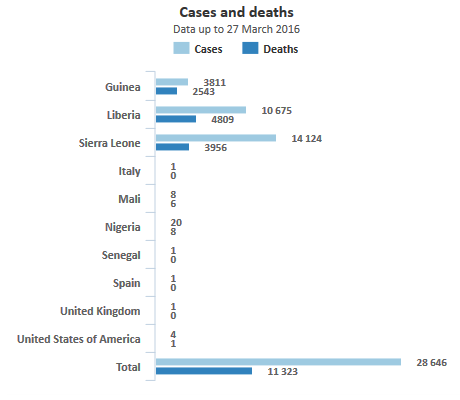
\includegraphics[width=0.8\textwidth]{ebola.png}
			\caption{Excerpt from \cite{who}.}
			\label{fig:ebola}
		\end{figure}

		R offers various data import options. The most useful I have found were \code{read.csv}\footnote{Words in monospace font refer to R commands. The cheat sheet at the end of the tutorial lists most of those used in this document.} to import csv data and \code{read.fwf} to import fixed-width data. To demonstrate, figure~\ref{fig:data} shows what csv (delimited) and fixed-width data look like side by side.
		\begin{figure}[h]
			\centering
			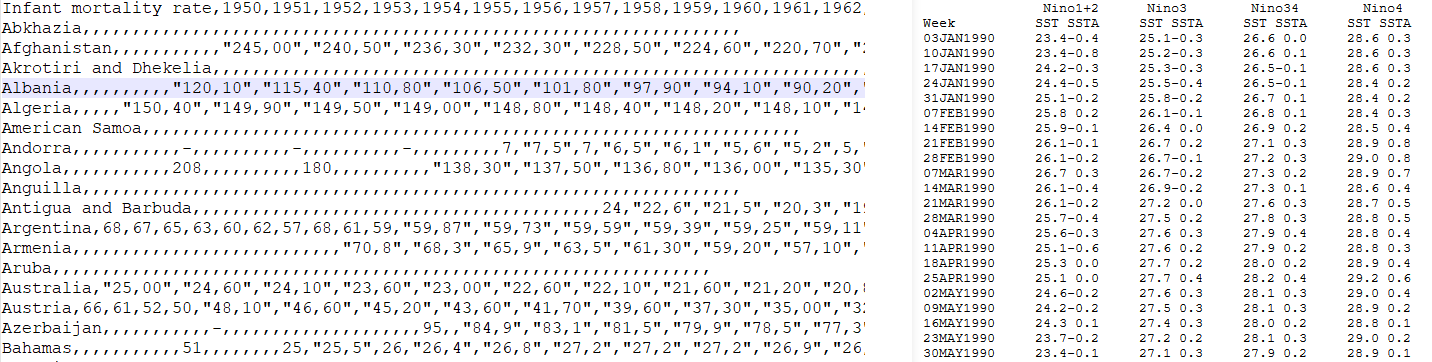
\includegraphics[width=1.0\textwidth]{data.png}
			\caption{Delimited data (left) and fixed-width data (right).}
			\label{fig:data}
		\end{figure}

		Go ahead and load your small csv into R with \code{read.csv('C:/......data.csv', header=TRUE)}. To avoid messing with default working folder in R settings, I recommend always using the full absolute file path (i.e. starting with C:). Note that you should use the \emph{forward slash "/"} as a path separator, even on Windows. The second parameter, \code{header=TRUE}, tells R that the first line in your file corresponds to the column headers, not actual data. You can then use the function \code{pie(counts, labels)} to produce a pie chart. However, as shown below, a naive approach might displease.
		\begin{minted}[breaklines]{R}
> ebola = read.csv('D:/megha/Documents/r-tutorial/ebola.csv', header=TRUE)
> ebola
                   Country Deaths
1                   Guinea   2543
2                  Liberia   4809
3             Sierra Leone   3956
4                     Mali      6
5                  Nigeria      8
6 United States of America      1
> pie(ebola)
Error in pie(ebola) : 'x' values must be positive.
		\end{minted}

		You might be scratching your head and wondering which part of 2543 or 6 is not positive, and you'd be justified to do so. Here, one must dive into computer programming concerns to understand what is going on. The "not positive" message hints at a problem with the format of the input data. Let's demonstrate:
		\begin{minted}[breaklines]{R}
> values = c(2543, 4809, 3956, 6, 8, 1
> labels = c('Guinea', 'Liberia', 'Sierra Leone', 'Mali', 'Nigeria', 'United States of America')
> pie(values, labels)	# works! produces figure 1.3
> typeof(values)
[1] "double"
> typeof(ebola)
[1] "list"
> class(values)
[1] "numeric"
> class(ebola)
[1] "data.frame"
> class(ebola$Country)
[1] "factor"
> class(ebola$Deaths)
[1] "integer"
> pie(ebola$Deaths, ebola$Country)	# works too now!

		\end{minted}
		\begin{figure}[h]
			\centering
			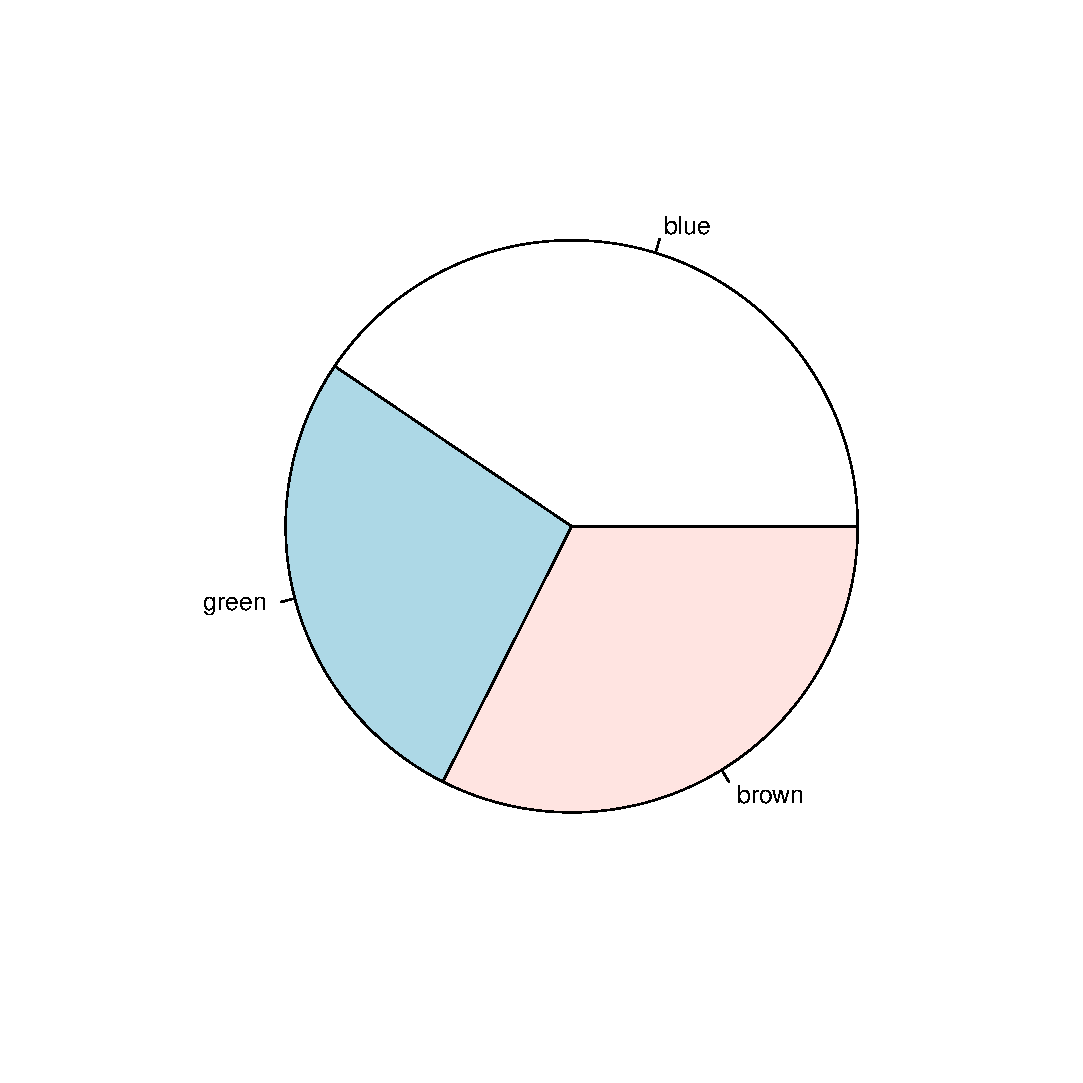
\includegraphics[width=0.8\textwidth]{pie.eps}
			\caption{Ebola deaths in 2015-2016 by country.}
		\label{fig:pie}
		\end{figure}

		Technically, \code{read.csv} returns a \code{data.frame}, while \code{pie} only accepts numbers. Let's take a painful tangent into R types that will hopefully help you later on.

		\begin{tcolorbox}[title=R types]
			\begin{tabularx}{\textwidth}{>{\bfseries}l X}
Logical: & TRUE or FALSE\\[0.2cm]
Numeric: & real, by the math definition (ex. 12.3). Double is a numeric with better precision.\\[0.2cm]
Integer: & integer, by the math definition (ex. 12).\\[0.2cm]
Character: & text of any length\\[0.2cm]
Factor: & a type that represents a \gls{dv}\\[0.2cm]
Ordered: & a type that represents an \gls{ov}\\[0.2cm]
List: & a 1D collection of "things" (may be strings, numbers, or a mix of them)\\[0.2cm]
Vector: & a 1D collection of things of \emph{one type}\\[0.2cm]
Matrix: & a 2D collection of things of \emph{one type}\\[0.2cm]
Array: & a nD collection of things of \emph{one type}\\[0.2cm]
Data Frame: & a (mostly) 2D collection of things, where each column can be of a different type
			\end{tabularx}
			For future reference, Quick R gives an excellent introduction on the subject~\cite{quickr}. You can convert a variable to anything reasonable (R will turn "2" into an integer, but not "abc") using the host of \code{as.xyz} functions.
		\end{tcolorbox}
		\begin{tcolorbox}[title=Accessing collection elements]
			Let's say you have a data frame, for example your ebola deaths by country data:
			\begin{minted}[breaklines]{R}
> ebola
                   Country Deaths
1                   Guinea   2543
2                  Liberia   4809
3             Sierra Leone   3956
4                     Mali      6
5                  Nigeria      8
6 United States of America      1
			\end{minted}
			Notice how the line with "Country" and "Deaths" is not numbered in the output? It means R is aware it's a header and not data. Data frame columns can be accessed by their name using the \code{\$} operator, like so:
			\begin{minted}[breaklines]{R}
> ebola$Country
[1] Guinea                   Liberia                  Sierra Leone            
[4] Mali                     Nigeria                  United States of America
6 Levels: Guinea Liberia Mali Nigeria ... United States of America
			\end{minted}
			If you want to access lines, you can use the \code{[row, column]} operator, like so:
			\begin{minted}[breaklines]{R}
> ebola[1,]
  Country Deaths
1  Guinea   2543
> ebola[1,2]
[1] 2543
			\end{minted}
			While the \code{\$} operator is exclusive to data frames, the \code{[]} is used for all collections. Vectors, lists, matrices and arrays can be accessed with the \code{[index]} operator for 1D structure, \code{[row, column]} operator for 2D structures, and \code{[i, j, k...]} for nD structures.

			In the case you want to access several items at once, you can use a colon inside the brackets, i.e. \code{[begin:end]} like so:
			\begin{minted}[breaklines]{R}
> ebola[1:3,]
       Country Deaths
1       Guinea   2543
2      Liberia   4809
3 Sierra Leone   3956
			\end{minted}
		\end{tcolorbox}

		Now that we have our basic pie chart, you might be thinking, "That squiggle on the right with the tiny pie slices is quite unseemly". In addition, you might want to tweak other aspects of the graph, like adding a title or choosing colors. We will discuss common graph properties in a following section, to keep it all in the same place. Let's just deal with the pie-chart specific problem of small slices here (I reiterate, you should run away, run away into the arms of a bar chart.), and add a percent annotation, as that is a common occurence. R does not offer an option to deal with small slices out of the box (probably because it tells you in its own manual to use bar charts instead), so let's just manually tweak the labels:
		\begin{minted}[breaklines]{R}
> labels = as.character(ebola$Country)
> labels[4]='Others'
> labels[5:6]=''
> labels
[1] "Guinea"       "Liberia"      "Sierra Leone" "Others"       ""            
[6] ""
> percents = ebola\$Deaths/sum(ebola\$Deaths)*100
> percents
[1] 22.458712355 42.471076570 34.937737349  0.052989490  0.070652654
[6]  0.008831582
> percents[4] = sum(percents[4:6])
> percents
[1] 22.458712355 42.471076570 34.937737349  0.132473726  0.070652654
[6]  0.008831582
> percents = round(percents, 2)
> percents
[1] 22.46 42.47 34.94  0.13  0.07  0.01
> labels[1:4] = paste(labels[1:4], percents[1:4], '\%')
> labels
[1] "Guinea 22.46 %"       "Liberia 42.47 %"      "Sierra Leone 34.94 %"
[4] "Others 0.13 %"
> pie(ebola\$Deaths, labels)
		\end{minted}
		Hacky, but it works, and no more time should be dedicated to pie charts, so let's move on.

		\subsection{Bar chart}
	A bar chart, sometimes called a line graph, is used to represent a \gls{dv}, and the bars \emph{do not touch}. As an example, data on infant mortality by country can be found at \href{https://docs.google.com/spreadsheets/d/1OHMMuHbSFKDolNHXsmgHYlkjSKfAZyyY1P-ddMu_Fz0/pub}{Gapminder}~\cite{gapminder}. If you simply \code{read.csv} the file you just downloaded and converted to csv using your favorite Spreadsheet software, and then examine the structure of your data inside R, you might notice the somewhat strange following occurence:
	\begin{minted}[breaklines]{R}
> infant = read.csv('D:/megha/Documents/r-tutorial/infant.csv', header=TRUE)
> class(infant)
[1] "data.frame"
> str(infant)
'data.frame':   260 obs. of  217 variables:
 $ Infant.mortality.rate: Factor w/ 260 levels "Abkhazia","Afghanistan",..: 1 2 3 5 6 7 8 9 10 11 ...
 $ X1800                : int  NA NA NA NA NA NA NA NA NA NA ...
 $ X1801                : int  NA NA NA NA NA NA NA NA NA NA ...
# ...
 $ X1861                : int  NA NA NA NA NA NA NA NA NA NA ...
 $ X1862                : Factor w/ 11 levels "",".","110","131",..: 1 1 1 1 1 1 1 1 1 1 ...
 $ X1863                : Factor w/ 13 levels "",".","106","113",..: 1 1 1 1 1 1 1 1 1 1 ...
# ... 
	\end{minted}

	Wait, what? The country is of type factor, we all agree on that, but infant mortality rate for 1862 is a factor? Using good ol' Notepad or a better text editor, open your csv and scroll around, you should spot the problem illustrated in figure~\ref{fig:welcome}.
	\begin{figure}[h]
		\centering
		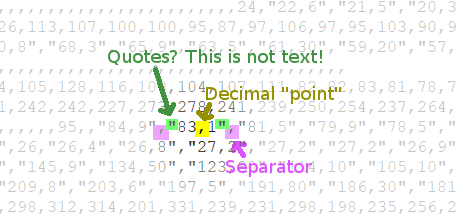
\includegraphics[width=1.0\textwidth]{welcometotherealworld.png}
		\caption{Welcome to the real world. CSV sucks internationally.}
	\label{fig:welcome}
	\end{figure}

	In other languages, like French for instance, the decimal "point" is a comma, and therefore the "comma-separated" part of comma-separated value leads to some issues. Other gems in this data include "-" for I assume missing data, and some lonely dots, assuming again, for missing data. Gods forbid the authors hit a snag while importing data and their software didn't warn them something foul was afoot and they just pasted it in the global csv without noticing. (This is why science should be in databases. Real databases. They don't let you put a dash in a number field, they just don't.)

	Thankfully, \code{read.csv} comes with some handy options. You can see them all in the manual by typing \code{?read.csv} in a R console. So, we need to tell R that our \code{dec} point is a comma, and dash and dot stand for missing data, i.e. \code{na.strings}. Technically, R also thinks that things surrounded by quotes are text, but is smart enough to automatically check if the "text" looks like a number and, if it does, it converts it automatically to a number. You therefore get the appropriate following:
	\begin{minted}[breaklines]{R}
> infant = read.csv('D:/megha/Documents/r-tutorial/infant.csv', header=TRUE, dec=",", na.strings=c('-', '.'))
> str(infant)
'data.frame':   260 obs. of  217 variables:
 $ Infant.mortality.rate: Factor w/ 260 levels "Abkhazia","Afghanistan",..: 1 2 3 5 6 7 8 9 10 11 ...
 $ X1800                : int  NA NA NA NA NA NA NA NA NA NA ...
 $ X1801                : int  NA NA NA NA NA NA NA NA NA NA ...
 # ...
	 \end{minted}

	A barplot is relatively straightforward to produce with R, but we will see all "common" (imho) plot options here, so tie your winter hat down with wire, you'll be sitting here a while.  Let's start by simply plotting infant mortality rate by country. To keep the plot readable, let's choose a subset of G8 countries: Canada, France, Germany, Italy, Japan, Russia, United Kingdom and United States of America. Let's also start by studying the mortality rate in 2000. First, we will select each of the countries by its row number, then we will stitch the G8 back together with a function called \code{rbind}, which binds data frames together by row, as long as all data frames have the same columns.
	\begin{minted}[breaklines]{R}
> canada = infant[38,]
> france = infant[77,]
> germany = infant[83,]
> italy = infant[109,]
> japan = infant[111,]
> russia = infant[186,]
> uk = infant[240,]
> usa = infant[241,]
> g8 = rbind(canada, france, germany, italy, japan, russia, uk, usa)
	 \end{minted}

	Producing a barplot now is easy:
	\begin{minted}[breaklines]{R}
> barplot(g8$X2000, names.arg=g8$Infant.mortality.rate)
	\end{minted}
	\begin{figure}[h]
		\centering
		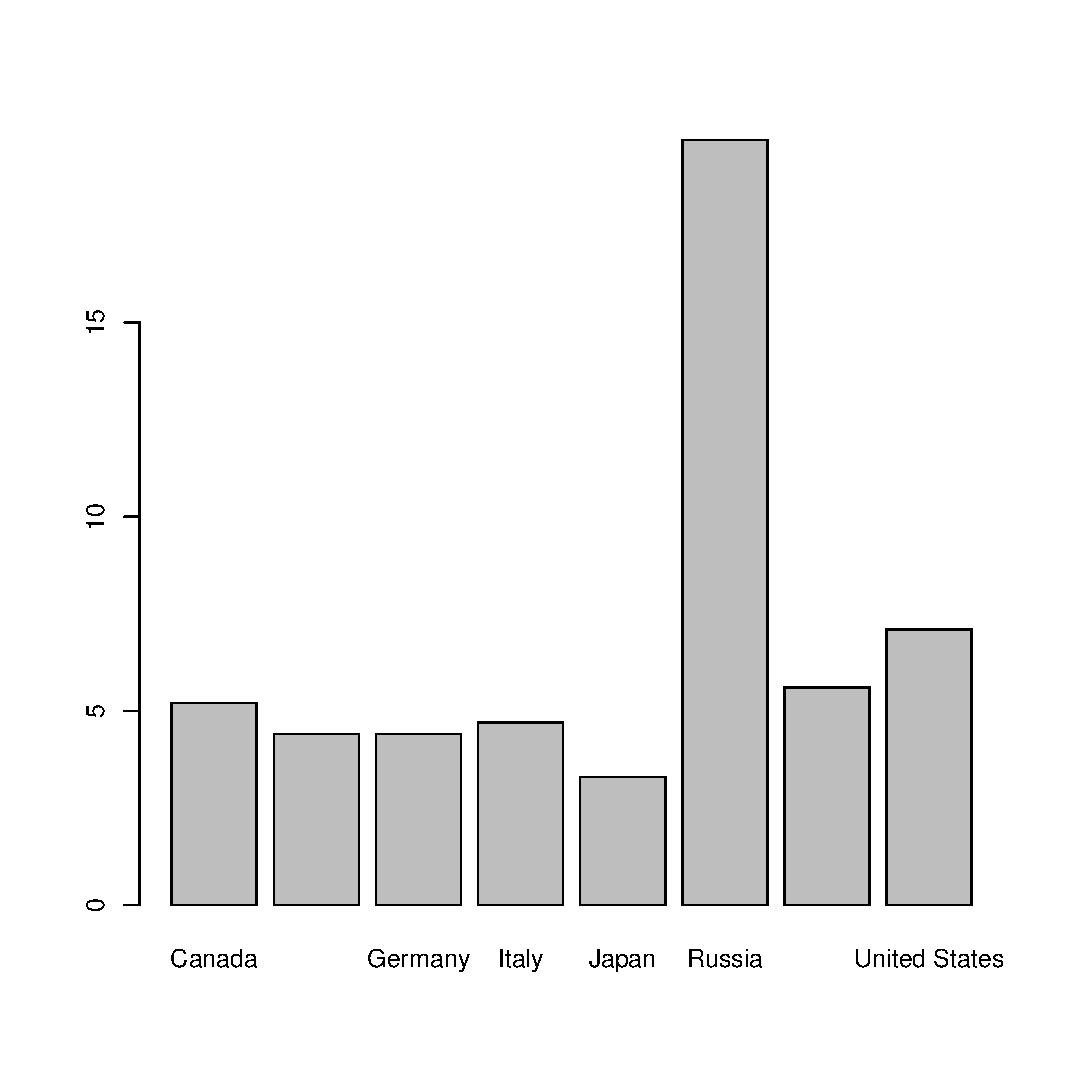
\includegraphics[width=1.0\textwidth]{barsimple.eps}
		\caption{Simplest bar plot: infant mortality rate per country.}
	\label{fig:simplebar}
	\end{figure}

	Several things are wrong with this graph. Glaringly, a bar should not extend beyond its axis. Axes are set as plot options with \code{xlim} and \code{ylim}. Also, should you want a box around the graph, \code{bty} takes care of that. Usually. Bar plots are special and you need to all an extra function after your plot appears. See all graph options with \code{?par}, which we will use a lot more as we customize our graphs.
	\begin{minted}[breaklines]{R}
barplot(g8$X2000, names.arg=g8$Infant.mortality.rate, ylim=c(0,20), bty='o')	# why oh why won't bty work like everywhere else!
box()
	\end{minted}
	\begin{figure}[h]
		\centering
		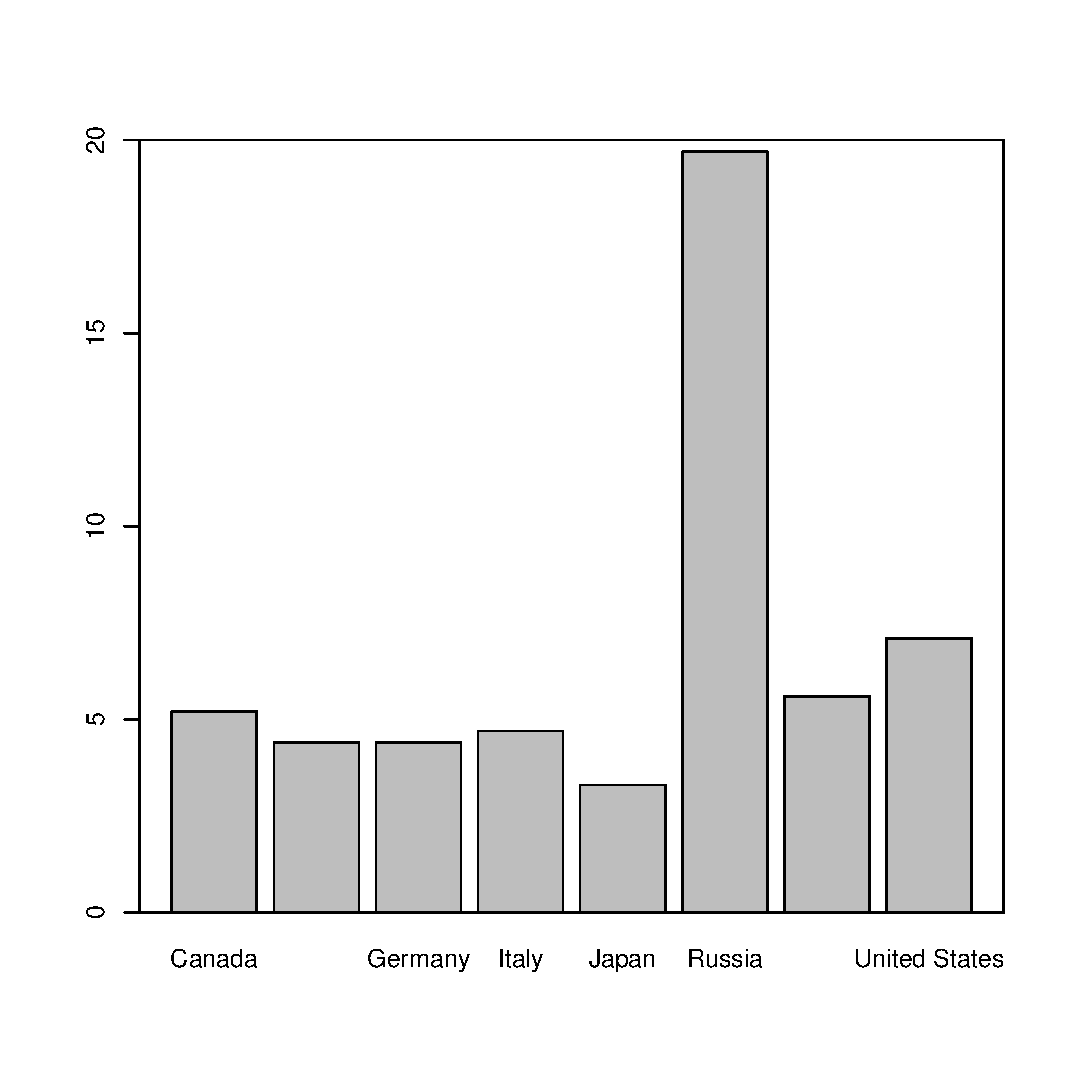
\includegraphics[width=1.0\textwidth]{baraxis.eps}
		\caption{Simple bar plot: infant mortality rate per country, axis set.}
		\label{fig:baraxis}
	\end{figure}

	You probably also want all country names to show up. Easiest way to do that is to tilt the axis label text. Enter \code{par}, used \emph{before} your graph function to set general settings. For this next iteration, let's do a few things at once. First, let's make all labels perpendicular to their axis with \code{par} and \code{las}. Let's also demonstrate color manipulation by making each country's bar the dominant color on their flag (this might lead to arbitrary choices) with \code{col}.
	\begin{minted}[breaklines]{R}
> colors = c('red', 'blue', 'black', 'green', 'white', 'snow', 'purple', 'purple4')
> par(las=2)		# axis labels: perpendicular
> barplot(g8$X2000, names.arg=g8$Infant.mortality.rate, ylim=c(0,20), col=colors)
> box()
	\end{minted}

	\begin{tcolorbox}[title=Colors in R, parbox=false]
Colors in R can be specified by their names, if they are among R's list of approved colors, which you can see by calling \code{colors()}.

A more visually helpful version can be found at \href{http://research.stowers.org/mcm/efg/R/Color/Chart/}{Color Chart}~\cite{rcolors} which, incidentally, has other fascinating references about the use of color in science (good vs. bad color ramps, color blindness considerations).

Additionally, colors can be specified in other formats like \code{\#RRGGBB} where 00 $\leq$ color $\leq$ FF. These values can be found with graphics software or off a color generator on the internet.

Finally, if color space is a factor, additional functions exist: \code{rgb}, \code{hsv}, \code{hcl}, \code{gray} and \code{rainbow}.
	\end{tcolorbox}

	\begin{figure}[h]
		\centering
		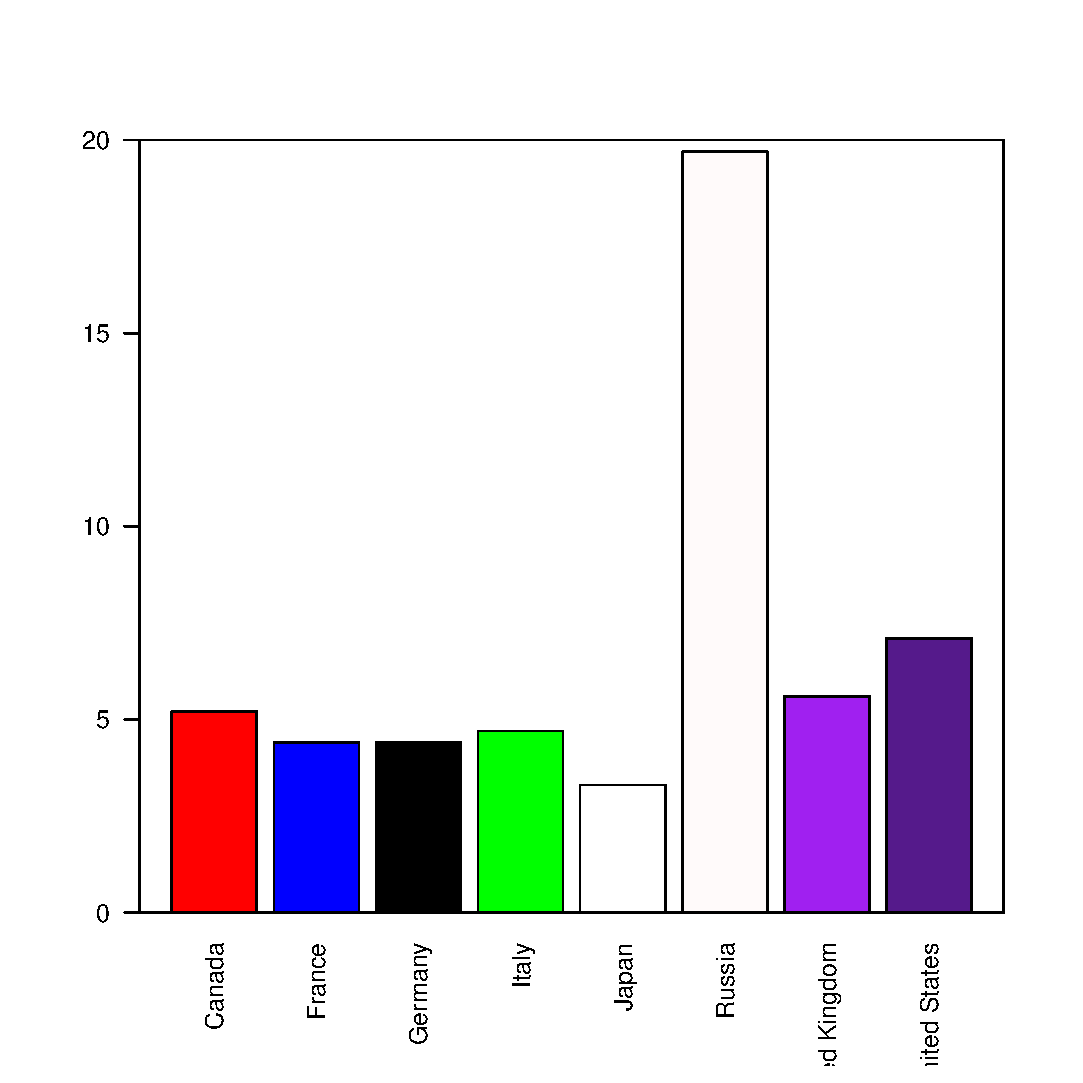
\includegraphics[width=1.0\textwidth]{barpsych.eps}
		\caption{Psychedelic bar plot: infant mortality rate per country, axis set, labels perpendicular, colors.}
		\label{fig:barpsych}
	\end{figure}

With the country names printed at the vertical, they are running out of space at the bottom of the graph. More margin is needed there. Figures have two types of margins in R: outer and inner. The inner margin is used to draw the figure title and the axis ticks and labels and can be set in inches with \code{mai=c(bottom, left, top, right)} or in lines with \code{mar=c(bottom, left, top, right)}. The outer margin is outside the figure; it makes more sense when several plots are displayed together, as we will do a few exercises down the line. The outer margin as well can be set in inches with \code{omi=c(bottom, left, top, right)} or in lines with \code{oma=c(bottom, left, top, right)}. As for the appropriate margin necessary to display the full country name, that's a matter of trial and error. Starting with the current parameters' value of inner margin, I found that a value of 8 worked well.
	\begin{minted}[breaklines]{R}
par()$mar
[1] 5.1 4.1 4.1 2.1
> par(mar=c(8, 4.1, 4.1, 2.1))
> barplot(g8$X2000, names.arg=g8$Infant.mortality.rate, ylim=c(0,20), col=colors)
> box()
	\end{minted}

Now, bar charts often use stacked bars. For example, let's use cancer rates \cite{cancer}. This data includes number of cases and number of deaths by sex and cancer type. If the thing you would most like to compare is the number of cancer by type, you would stack the sexes into one bar, and make one bar for new cases and one bar for deaths.  Data can most easily be copy-pasted into a Spreadsheet software from Table 1 of  the peer-reviewed article version of the report \cite{siegel_cancer_2018}. After removing sum lines and columns, removing the thousand separator, tweaking header names, saving as csv and importing into R, you can produce your bar chart:
	\begin{minted}[breaklines]{R}
> cancer = read.csv('C:/Users/Myriam/Documents/r-tutorial/cancer.csv')
> cancer
                              cancer cases_male cases_female deaths_male deaths_female
1                             Tongue      12490         4620        1750           760
2                              Mouth       7980         5600        1770           880
...
47 Other & unspecified primary sites      16520        15290       23950         20610
> str(cancer)
'data.frame':   47 obs. of  5 variables:
 $ cancer       : Factor w/ 47 levels "Acute lymphocytic leukemia",..: 41 19 32 27 10 38 36 9 34 3 ...
 $ cases_male   : int  12490 7980 14250 2440 13480 16520 ...
 $ cases_female : int  4620 5600 3340 820 3810 9720 ...
 $ deaths_male  : int  1750 1770 2480 1280 12850 6510 ...
 $ deaths_female: int  760 880 750 360 3000 4290  ...
	\end{minted}


	\subsection{Histogram}
	\subsection{Line graph}
	\subsection{Scatter graph}
	\subsection{Box and whiskers graph}
	\section{Numbers}
	\subsection{Center}
	\subsubsection{Mean}
	\subsubsection{Median}
	\subsubsection{Mode}
	\subsection{Dispersion}
	\subsubsection{Range}
	\subsubsection{Variance}
	\subsubsection{Standard deviation}
	\subsubsection{Coefficient of variation}
	\subsubsection{Quartiles and percentiles}
	\subsection{Shape}
	\subsubsection{Skewness}
	\subsubsection{Kurtosis}
	\subsubsection{L-moments}

\chapter{Probabilities}
	\section{Factorial}
	\section{Combinations}
	\section{Permutations}
	\section{Probability Mass/Density Function}

\chapter{Statistics}
	\section{Binomial distribution}
	\section{Multinomial distribution}
	\section{Poisson distribution}
	\section{Inverse binomial distribution}
	\section{Hypergeometric distribution}
	\section{Normal distribution}
	\section{Exponential distribution}
	\section{Gamma distribution}
	\section{c2 distribution}
	\section{Fisher-Snedecor distribution}
	\section{Student’s law}

\chapter{Inferential statistics}
	\section{Student’s test}
	\section{Student’s paired test}
	\section{Bartlett’s test}
	\section{Single-factor ANOVA}
	\section{c2 test}
	\section{Wilcoxon-Mann-Whitney test}
	\section{Kolmogorov-Smirnov test}
	\section{Kruskal-Wallis test}
	\section{Pearson’s test}
	\section{Spearman’s test}
	\section{Kendall’s test}
	\section{Simple linear regression}
	\section{Multiple linear regression}

\chapter{Cheat sheet}

	\section{Plumbing}
\begin{tabbing}
?~~~~~~~~~~~~~ \= ?exact\_function\_name \\
?? \> ??keyword \\
typeof \> typeof(R\_variable) \\
class \> class(R\_variable) \\
str \> str(R\_variable) \\
colnames \> colnames(R\_variable) \\
as.integer \> as.integer(R\_variable)
\end{tabbing}

	\section{Data import and export}
\begin{tabbing}
read.csv~~~~ \= read.csv('delimited\_data.csv', header=TRUE, sep=",", dec=".") \\
read.fwf \> read.fwf('fixed\_width\_data.txt', widths=c(10, 5, 4), header=TRUE, skip=2) \\
write.csv \> write.csv(R\_variable, file='desired\_file\_name.csv', row.names=FALSE, append=FALSE)
\end{tabbing}

\printbibliography

\printnoidxglossaries

\end{document}